\documentclass[12pt, letterpaper]{report}
\let\cleardoublepage\clearpage
\setlength{\headheight}{14.5pt}


%---------PACKAGES-------------
\usepackage{indentfirst}
\usepackage[utf8]{inputenc}
\usepackage[T1]{fontenc}
\usepackage[margin=1in]{geometry}
%\usepackage{1modern}
\usepackage{setspace}
\usepackage{graphicx}
\usepackage{float}
\usepackage{caption}
\usepackage{booktabs}
\usepackage{amsmath, amssymb}
%\usepackage{sinuitx}
\usepackage{hyperref}
\usepackage{fancyhdr}
\usepackage{lineno}
\usepackage{tocloft}
\usepackage{titlesec}
\usepackage{xcolor}
\usepackage{listings}
\usepackage{cite}

%----------HYPERREF-----------
\hypersetup{
    colorlinks=true,
    linkcolor=blue,
    citecolor=blue,
    urlcolor=blue,
    pdftitle={Foundation Fix -- Engineering Report},
    pdfauthor={
        Akhil Nandhakumar, Allyson Lay, Dalen Avrin Smith, Elizabeth Yancey,
        Emma Shin, Harmeet Singh, Ival Momoh, Jay Kim, Richard Tokiyeda, Victoria Sun
    }
}
\pagestyle{fancy}
\fancyhf{}
\fancyhead[L]{\textit{Theta Beta Engineer Project}}
\fancyhead[R]{\textit{Draft -- 0.1}}
\fancyfoot[C]{\thepage}

\title{
    \textbf{Theta Beta Engineer Project Report}\\[0.5em]
    \large Foundation Color Identifier and Dispenser\\
    University of California, Irvine
}
\author{
    Akhil Nandhakumar, Allyson Lay, Dalen Avrin Smith,\\
    Elizabeth Yancey, Emma Shin, Harmeet Singh, Ival Momoh,\\
    Jay Kim, Richard Tokiyeda, Victoria Sun
}
\date{November 17, 2025}

\begin{document}

    \maketitle
    \pagenumbering{roman}

    \linenumbers

    \tableofcontents
    \listoffigures
    \listoftables
    \newpage

    \pagenumbering{arabic}

    %===========================ABSTRACT===========================
    \chapter{Abstract}
    
    
    The Foundation Identifier and Dispenser aims to develop a machine that is able to
    extract samples from a picture of a human to determine the shade of their skin, allowing
    the machine to dispense a corresponding foundation shade. The results produced
    should be both accurate and reproducable. Equipped with computer vision libraries
    and color correction algorithms, the system allows the user to take an picture alongside 
    a reference color sheet, which has colors of known values. These captured values are 
    processed to correct both camera bias, and lighting correction so that results
    may remain consistent regardless of lighting conditions during image capture. The system
    converts RGB values to LAB values, which are higher in accuracy in physical color 
    mixing, as opposed to RGB, which is used to describe pixel colors. The program calculates
    how much of each color is needed to recreate the user's skin pigment. These pigments are
    then dispensed via a mechanical system comprised of a Raspberry Pi, servo motors, and 
    syringes. This project demonstrates an application of computer vision in the cosmetic
    market to alleviate the burden of overconsumption and promote inclusivity. 

    %===========================INTRODUCTION===========================

    \chapter{Introduction}

    \section{Research}
    \subsection{Background of Problem}
    
    Testing foundation colors can be a frustrating experience for many, who are unable to find
    the perfect balance. At the end of the day, no line of foundation can realistically
    provide colors that cater to every possible skin tone. The seemingly unresolvable desire
    for a perfect shade leads many makeup users to spend hundreds on shades that are "close enough."
    This leads to lots of waste, not just in money, but in bottles thrown out after purchase because
    the match was ultimately unsatisfying. 
    the match was ultimately unsatisfying. 

    The beauty industry produces 120 billion packaging units per year and 95\% of this these units
    are discarded, as opposed to recycled \cite{SmithS}. In addition, traditionally a custom skin matched foundation 
    can cost anywhere from \$60-100 per bottle, which leaves the consumers with the dilemma of whether they should
    take the gamble on the bottle that's just almost right versus breaking their wallet on a hand matched bottle. 
    Our custom mixer machine offers the same accuracy in skin tone while also promoting cheaper makeup,
    sustainability, and waste-reduction. 
    sustainability, and waste-reduction. 

    Our foundation color picker abandons the concept of creating a set of discrete skin tones to choose from,
    instead, opting for custom mixed shades depending on the skin color detected by a picture. 
    It also offers the unique ability to sample a shade without having to commit to a full sized bottle. 


    \subsection{Existing Solutions}
    BoldHue provides an option for an AI powered foundation mixer. It matches skin tone through a smart wand 
    that detects color. What they promised was millions of shades and the ability to store user's shades in profiles.
    However, their color detection methods provide room for lots of error because color isn't percieved the same depending
    on the lighting of the room, as well as the high cost of their machine. 
    on the lighting of the room, as well as the high cost of their machine. 

    Our product will have built in lighting correction that removes biases from the camera and uses the Macbeth Color Reference sheet 
    as a set of control colors. The reference sheet is what will allow the machine to recallibrate it's understanding of what colors
    are being percieved. 
    

    \section{Design Choices}
    \subsection{Past Considerations and Scrapped Plans}

    \textbf{Off-the-Shelf Syringe Pump System}

    An early design decision we explored was to use commercially available syringe pump 
    system available for purchase from a third party. This idea was ultimately abandoned due
    to bulkiness of commercial pumps, as well as high cost. Although designing our own pump
    system required more work from our mechanical team to design the system from scratch,
    relying on an existing system would have limited our freedom, increased our costs, and 
    taken away from the educational value of the project. Designing a custom syringe pump
    offered hands-on learning experiences in CAD design. 
    \bigbreak

    \textbf{Quick-Swap Syringe Mounting Attachment}

    We also considered designing the Syringe housing to allow users to detatch and fill syringes 
    in between uses. This feature was ultimately unnecessary as the syringes don't need to be 
    manually pumped. As long as the moters can rotate the opposite direction, the syringes
    dont have to be removed to retract. The final design eliminated the syringe-swapping mechanism
    in favor of refilling via holding a paint vial under the syringe and letting the machine 
    retract the pump to draw in fluid. 
    \bigbreak

    \textbf{Single-Piece Printed Housing}

    Our initial housing was a single piece. However, most 3D printers that were available have a 
    maximum build volume of 256 mm x 256 mm x 256 mm, and the housing dimensions we had for the 
    initial design was too close to this limit. Printing the structure in a single piece also 
    risks expensive failed prints, warping, and geometric constraints. We shifted to a housing 
    unit comprised of three interlocking sections, with custom brackets to join the segments securely. 

    %===========================HARDWARE DESIGN===========================

    \chapter{Hardware Design and Specifications}

    \section{First Iteration}
    \subsection{Initial CAD Model and Hand Sketches}
    \begin{figure}[H]
        \centering
        \includegraphics[width=0.6\textwidth]{assets/first_it/ME_init_sketch_housing.png}
        \caption{First Sketch: Housing}
    \end{figure}
    \begin{figure}[H]
        \centering
        \includegraphics[width=0.4\textwidth]{assets/first_it/ME_init_cad_housing2.png}
        \includegraphics[width=0.4\textwidth]{assets/first_it/ME_init_cad_housing2.png}
        \caption{First CAD Models: Housing}
    \end{figure}
    \begin{figure}[H]
        \centering
        \includegraphics[width=0.8\textwidth]{assets/first_it/ME_init_sketch_dispenser.png}
        \caption{First Sketch: Dispenser Systems}
    \end{figure}
    \begin{figure}[H]
        \centering
        \includegraphics[width=0.8\textwidth]{assets/first_it/ME_init_cad_dispenser.png}
        \caption{First CAD Models: Dispenser Systems}
    \end{figure}

    Our first CAD Models were very simple and provide the most general idea 
    we had at our projects conception. We made large changes to the design of
    the housing because the dimensions would have been much wider if we lined
    the syringes up, as shown in Figures 3.1 and 3.2.

    The preliminary sketch we have of the dispenser system has stayed consistent
    throughout development. 
    \pagebreak
    
    \section{Second Iteration}
    
    \subsection{Updated CAD Models}
    \textbf{\textit{Assembly}}
    \begin{figure}[H]
        \centering
        \includegraphics[width=0.8\textwidth]{assets/second_it/ME_full_assembly.png}
        \caption{Second Iteration: Full Assembly}
    \end{figure}
    \begin{figure}[H]
        \centering
        \includegraphics[width=0.8\textwidth]{assets/second_it/ME_exploded.png}
        \caption{Second Iteration: Exploded View}
    \end{figure}
    \pagebreak

    \textbf{\textit{Housing}}
    \begin{figure}[H]
        \centering
        \includegraphics[width=0.4\textwidth]{assets/second_it/ME_housing_skeleton.png}
        \includegraphics[width=0.32\textwidth]{assets/second_it/ME_housing_walls.png}
        \caption{Second Iteration: Housing Skeleton and Walls}
    \end{figure}

    The housing skeleton is what holds the syringes in place while the walls create an enclosure
    so that the internal structure may be protected and hidden from users. The main concern with 
    this iterations design was with the housing skeleton's stability. Since we were 3D printing 
    all parts for the demo, the empy spaces could be flimsy, so the final iteration includes a 
    redesign. 

    \textbf{\textit{Dispenser}}
    \begin{figure}[H]
        \centering
        \includegraphics[width=0.4\textwidth]{assets/second_it/ME_guide_shaft_bracket.png}
        \includegraphics[width=0.25\textwidth]{assets/second_it/ME_syringe_holder_bracket.png}
        \includegraphics[width=0.25\textwidth]{assets/second_it/ME_syringe_plunger_bracket.png}
        \caption{Second Iteration: Brackets for Dispenser System}
    \end{figure}

    These brackets hold and control the dispenser system. The first L-shaped Bracket holds 
    the guide shaft in place. The other two are for stabilizing and pushing the syringe 
    plunger down. This second iteration is missing one of the parts but it will be shown 
    in the next section, along with final drawings of all parts. 
   
    \pagebreak

    
    \subsection{Updated CAD Models}
    \textbf{\textit{Assembly}}
    \begin{figure}[H]
        \centering
        \includegraphics[width=0.8\textwidth]{assets/second_it/ME_full_assembly.png}
        \caption{Second Iteration: Full Assembly}
    \end{figure}
    \begin{figure}[H]
        \centering
        \includegraphics[width=0.8\textwidth]{assets/second_it/ME_exploded.png}
        \caption{Second Iteration: Exploded View}
    \end{figure}
    \pagebreak

    \textbf{\textit{Housing}}
    \begin{figure}[H]
        \centering
        \includegraphics[width=0.4\textwidth]{assets/second_it/ME_housing_skeleton.png}
        \includegraphics[width=0.32\textwidth]{assets/second_it/ME_housing_walls.png}
        \caption{Second Iteration: Housing Skeleton and Walls}
    \end{figure}

    The housing skeleton is what holds the syringes in place while the walls create an enclosure
    so that the internal structure may be protected and hidden from users. The main concern with 
    this iterations design was with the housing skeleton's stability. Since we were 3D printing 
    all parts for the demo, the empy spaces could be flimsy, so the final iteration includes a 
    redesign. 

    \textbf{\textit{Dispenser}}
    \begin{figure}[H]
        \centering
        \includegraphics[width=0.4\textwidth]{assets/second_it/ME_guide_shaft_bracket.png}
        \includegraphics[width=0.25\textwidth]{assets/second_it/ME_syringe_holder_bracket.png}
        \includegraphics[width=0.25\textwidth]{assets/second_it/ME_syringe_plunger_bracket.png}
        \caption{Second Iteration: Brackets for Dispenser System}
    \end{figure}

    These brackets hold and control the dispenser system. The first L-shaped Bracket holds 
    the guide shaft in place. The other two are for stabilizing and pushing the syringe 
    plunger down. This second iteration is missing one of the parts but it will be shown 
    in the next section, along with final drawings of all parts. 
   
    \pagebreak


    \section{Third Iteration}
 
    \subsection{Final CAD Models}
    \textbf{\textit{Assembly}}
    \begin{figure}[H]
        \centering
        \includegraphics[width=1\textwidth]{assets/third_it/ME_full_device_assembly.png}
        \caption{Final: Full Assembly \(Exploded\)}
    \end{figure}
    \pagebreak

    \textbf{\textit{Housing}}
    \begin{figure}[H]
        \centering
        \includegraphics[width=0.4\textwidth]{assets/third_it/ME_case_back_wall.png}
        \includegraphics[width=0.35\textwidth]{assets/third_it/ME_case_side_wall.png}
        \caption{Housing: Walls}
    \end{figure}
    \begin{figure}[H]
        \centering
        \includegraphics[width=0.4\textwidth]{assets/third_it/ME_case_lid.jpeg}
        \caption{Housing: Lid}
    \end{figure}
    \begin{figure}[H]
        \centering
        \includegraphics[width=0.8\textwidth]{assets/third_it/ME_case_skeleton_frame.png}
        \caption{Housing: Skeleton}
    \end{figure}

    The Housing walls were altered to include a slit because there are some screws in the 
    skeleton of the product that would press up against the walls if we kept the second iteration's
    design. The slit was created to give the screws space and ensure that the components inside 
    are not putting pressure on each other. 

    \pagebreak

    \textbf{\textit{Dispenser}}
    \begin{figure}[H]
        \centering
        \includegraphics[width=0.325\textwidth]{assets/third_it/ME_case_l_bracket.png}
        \includegraphics[width=0.375\textwidth]{assets/third_it/ME_l_bracket.png}
        \includegraphics[width=0.36\textwidth]{assets/third_it/ME_syringe_bracket.png}
        \includegraphics[width=0.35\textwidth]{assets/third_it/ME_plunger_bracket.png}
        \caption{Dispenser System : Brackets - for connecting to housing, guide shaft,
        stabilizing syringe, and pushing down syringe plunger}
    \end{figure}
    \begin{figure}[H]
        \centering
        \includegraphics[width=0.8\textwidth]{assets/third_it/ME_dispenser_mechanism_assembly.png}
        \caption{Dispenser System : Full assembly}
    \end{figure}

    The final design consists of four primary components: an L-bracket connecting the 
    dispenser to the casing, a secondary L-bracket securing the guide rod, 
    a syringe bracket that stabilizes and positions the syringe, and a plunger plate driven 
    by the lead screw to depress the syringe plunger.

    The final iteration incorporates several refinements across all components. 
    Mounting brackets and L-brackets were redesigned with rounded edges to increase 
    clearance between moving elements. The lower syringe bracket was modified to include 
    two vertical extrusions that act as contact surfaces for limit switches. Additionally, 
    mounting holes for fasteners were added throughout the assembly to improve 
    structural stability and ease of integration.
    \pagebreak

    \subsection{Final Manufacturing Drawings for Custom Parts}
    
    \begin{figure}[H]
        \centering
        \includegraphics[width=1\textwidth]{assets/third_it/ME_d_exploded_drawing.jpeg}
        \caption{Full Assembly Exploded View}
    \end{figure}
    \pagebreak

    \textbf{\textit{Housing}}
    \begin{figure}[H]
        \centering
        \includegraphics[width=1\textwidth]{assets/third_it/ME_d_Case_back.jpeg}
        \caption{Housing: Walls - Back}
    \end{figure}
    \begin{figure}[H]
        \centering
        \includegraphics[width=1\textwidth]{assets/third_it/ME_d_Case_Side.jpeg}
        \caption{Housing: Walls - Side}
    \end{figure}
    \begin{figure}[H]
        \centering
        \includegraphics[width=0.8\textwidth]{assets/third_it/ME_d_Case_lid.jpeg}
        \caption{Housing: Lid}
    \end{figure}
    \pagebreak
    
    \textbf{\textit{Dispenser}}
    \begin{figure}[H]
        \centering
        \includegraphics[width=1\textwidth]{assets/third_it/ME_d_Case_L_bracket.jpeg}
        \includegraphics[width=0.9\textwidth]{assets/third_it/ME_d_L_bracket.png}
        \caption{Dispenser System : L-Brackets}
    \end{figure}
    \pagebreak
    \begin{figure}[H]
        \centering
        \includegraphics[width=1\textwidth]{assets/third_it/ME_d_Syringe_bracket.png}
        \includegraphics[width=1\textwidth]{assets/third_it/ME_d_plunger_bracket.png}
        \caption{Dispenser System : Syringe Brackets}
    \end{figure}
    \begin{figure}[H]
        \centering
        \includegraphics[width=0.8\textwidth]{assets/third_it/ME_d_Dispenser_exploded.png}
        \caption{Dispenser System : Full assembly Exploded View}
    \end{figure}

    %===========================SOFTWARE DESIGN==========================

    \chapter{Software Design}

    \section{First Iteration}
    \subsection{Preliminary Diagrams and Psuedocode}
    \begin{figure}[H]
        \centering
        \includegraphics[width=0.8\textwidth]{assets/first_it/CS_userflow.png}
        \caption{Initial Flowchart for Control Logic}
    \end{figure}
    \begin{figure}[H]
        \centering
        \includegraphics[width=0.8\textwidth]{assets/first_it/CS_pseudocode1.png}
        \includegraphics[width=0.8\textwidth]{assets/first_it/CS_pseudocode2.png}
        \caption{Pseudocode: Image Processing Algorithms.}
    \end{figure}
    \begin{figure}[H]
        \centering
        \includegraphics[width=0.8\textwidth]{assets/first_it/CS_pseudocode3.png}
        \caption{Pseudocode: Embedded System.}
    \end{figure}

    The pseudocode shows our preliminary ideas for how the software would be 
    structured. It shows all the steps needed to turn Gamma Corrected RGB, 
    which is what the camera picks up, into values that represent the colors
    in the physical, non-digital world [2]. The algorithm is primarily based 
    linear algebra transformations and matrix operations [3]. 
    

    \subsection{Techstack}
    Frontend: React, Vite, Typescript, TailwindCSS, Lucide Icons
    
    Storage : IndexedDB (local storage)

    Hardware/OS/Hosting : Raspberry Pi (Linux, Pi Local Hosting)

    Computer Vision \& Data Science : OpenCV, NumPy, Pandas, Haar Cascades

    Languages : Typescript, Python

    Tooling : Git/Github
    
    \section{Second Iteration}
    \subsection{Lo-fi/Mid-fi Designs}
    \begin{figure}[H]
        \centering
        \includegraphics[width=0.4\textwidth]{assets/first_it/CS_ui-landing.png}
        \caption{Initial Figma Mockup: UI/UX - Landing page.}
    \end{figure}
    \begin{figure}[H]
        \centering
        \includegraphics[width=0.4\textwidth]{assets/first_it/CS_ui-load.png}
        \includegraphics[width=0.4\textwidth]{assets/first_it/CS_ui-color.png}
        \caption{Initial Figma Mockup: UI/UX - Loading the foundation shades.}
    \end{figure}

    \subsection{Basic Logic and Functionality}
    
    The backend service is responsible for two core tasks: analyzing a user’s 
    skin tone from an input image and triggering the dispenser system for a requested 
    foundation color. It is implemented as a Flask web API with three main endpoints: 
    '/analyze', '/dispense', and '/ping' \(app.py\). 
    \bigbreak
    
    \subsubsection{Skin Tone Analysis Pipeline \('/analyze'\)}
    
    \textbf{Image intake (frontend → backend) : }

    Frontend allows the user to view a live feed and takes a picture when it detects the face 
    reference sheet within the yellow box on the screen. The photo is sent to the '/analyze'
    endpoint. Backend strips, decods, and loads the data captured into an image object, which is
    saved for processing. 
    
    \textbf{Skin region extraction : }

    The image is converted to a NumPy RGB array and passed to '\texttt{define\_skin()}', which detects 
    and isolates skin pixels. this focuses the analysis on relevant skin regions instead of 
    the background.
    
    \textbf{Color space processing and lighting correction : }

    Skin samples are flattened into a matrix and normalized. '\texttt{gamma\_to\_linear()}'
    converts gamma corrected RGB values to linear RGB. '\texttt{lighting\_correction()}' corrects the for
    inconsistent lighting and the corrected RGB is converted to XYZ in '\texttt{linear\_to\_xyz()}' then
    to LAB in '\texttt{xyz\_to\_lab()}' [4].
    
    \textbf{Output color encoding : }

    The average LAB color is mapped to an approximate RGB value in '\texttt{lab\_avg\_to\_rgb()}' and 
    formatted as a hexadecimal color string. This hexadecimal string is returned as
    '\{"result":"<hex\_color>"\}' to the front end, which uses it for visualization for the user[5]. 
    \bigbreak

    \subsubsection{Dispensing Logic \(`/dispense`\)}
    
    Dispense accepts JSON payload containing the LAB code of the detected color. The endpoint 
    validates that the color is detected and prints a message to let the user know dispensing 
    has started. The endpoint is connected to the Raspberry Pi that drives the stepper motors 
    and pumps.
    \bigbreak

    \subsubsection{HealthHealth Check \(`/ping`\)}
    
    The `/ping` endpoint is a lightweight health-check route that returns 
    status updates. It allows the frontend to verify that the backend service 
    is alive and responsive without invoking the full analysis pipeline.     
    
    \subsection{Core Features of Algorithm}

    The color detection algorithm transforms raw camera input into a corrected, 
    device and lighting independent representation of the user's skin tone. This corrected color 
    is then mapped to a cosmetic shade. 

    \subsubsection{Macbeth Color Chart Reference Calibration}

    \begin{figure}[H]
        \centering
        \includegraphics[width=0.5\textwidth]{assets/final/macbeth.png}
        \caption{Macbeth Color Reference Sheet}
    \end{figure}

    The algorithm incorporates a Macbeth-style color chart for lighting and camera calibration.
    Known RGB or Lab reference values for each chart patch are compared to captured values:
    \begin{itemize}
        \item The color chart is detected and segmented from the image.
        \item We extract a sample from the middle of the patch.
        \item We correct the lighting and distortion
    \end{itemize}

    \subsubsection{Robust Skin Sampling from Facial Regions}

    A Haar-cascade face detector identifies the face region and we extract stable sampling zones 
    from the mask returned by the Haar-cascade. Regions of interest were defined as the forehead, 
    nose, and cheeks. Multiple points inside each region are collected to avoid shadows, 
    edges, or hair interference. These values are aggregated to produce a stable estimate of the 
    user's skin tone.

    \subsubsection{Gamma Correction and Linear RGB Conversion}

    Since cameras produce gamma-encoded RGB values, the algorithm applies a gamma-to-linear 
    transformation. Both chart colors and skin samples are linearized before calibration. 
    Working in linear RGB ensures that subsequent lighting corrections and color transformations are 
    physically meaningful.

    \subsubsection{Lighting Correction Using Chart Reference Data}

    A lighting correction is computed by comparing captured and reference chart patch colors. 
    This correction is applied uniformly to the sampled skin pixels, producing values that approximate 
    standardized, ideal lighting conditions.

    \subsubsection{Transformation into Lab Color Space}

    The corrected linear RGB values are converted into XYZ and then into Lab, 
    a device-independent and perceptually uniform color space. Multiple Lab samples from different 
    regions are averaged to form the final skin-tone vector.

    \subsubsection{Cosmetic Shade Selection and Hex Output}

    The final Lab vector is matched against a database of known cosmetic shades, each precomputed in Lab. 
    The system selects the shade with the smallest perceptual difference ($\Delta E$). 
    The algorithm returns the shade as: a hex code, corrected RGB, and Lab code.

    \subsubsection{Integration with Hardware Dispensing Logic}

    The selected shade is mapped to pigment ratios for the dispenser hardware. The backend provides:
    \begin{itemize}
        \item \texttt{/analyze}: accepts an image and returns the computed shade,
        \item \texttt{/dispense}: controls Raspberry Pi motors to dispense pigment.
        \item \texttt{/ping}: returns status updates and process health
    \end{itemize}


    \section{Third Iteration}
    \subsection{Final Product}

    \href{https://github.com/dalenas/foundation-fix/tree/main}{Foundation Fix Github} 


    %===========================ELECTRICAL ENGINEERING DESIGN===========================

    \chapter{Electrical Systems Design}

    \section{First Iteration}
    \subsection{Initial Wiring Diagrams}
    \begin{figure}[H]
        \centering
        \includegraphics[width=0.8\textwidth]{assets/first_it/EE_wiring.png}
        \caption{Preliminary Wiring Diagram}
    \end{figure}
    \subsection{Initial Power Calculations}
    \begin{table}[H]
        \centering
        \begin{tabular}{l l c}
            \toprule
            Parameter & Symbol & Value \\
            \midrule
            Phase Current & I & 0.7 \\
            Phase Resistance & R & 4.0 \\
            Phases & -- & 2 \\
            \bottomrule

        \end{tabular}
        \caption{Power Calculations}
        \label{tab:Electrical}
    \end{table}
    \[P_{motor}=2*I^2*R\]
    \[P_{motor}=2*(0.7)^2*4.0=3.92*5=19.6W\]
    \[P_{Raspberry Pi}=10W\]
    \emph{\[P_{total}=10+19.6=30W\]}

    


    \section{Second Iteration}
    \subsection{Circuit Building}

    \begin{figure}[H]
        \centering
        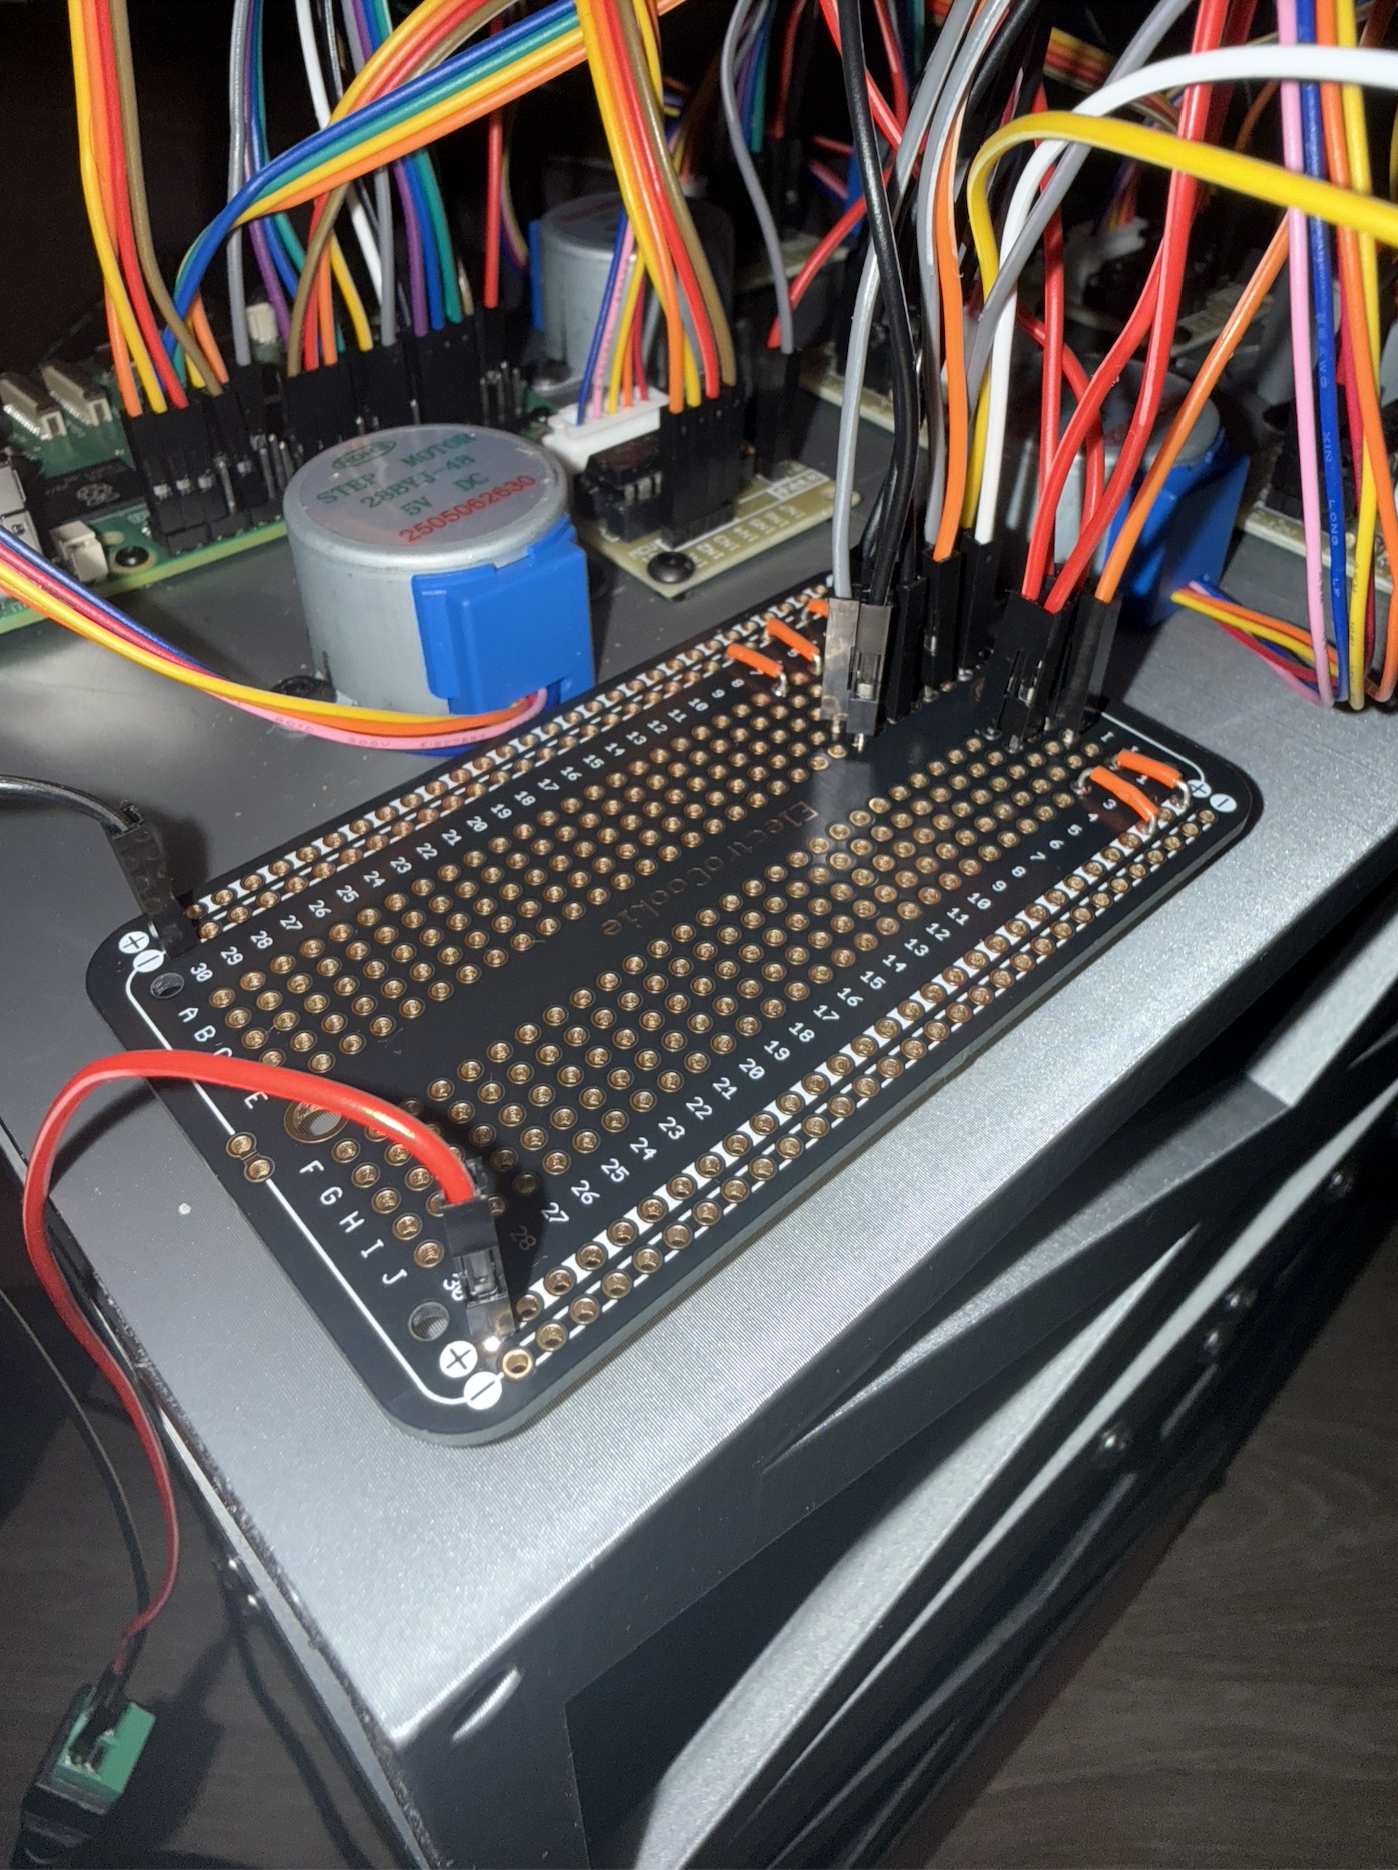
\includegraphics[width=0.35\textwidth]{assets/final/perf.png}
        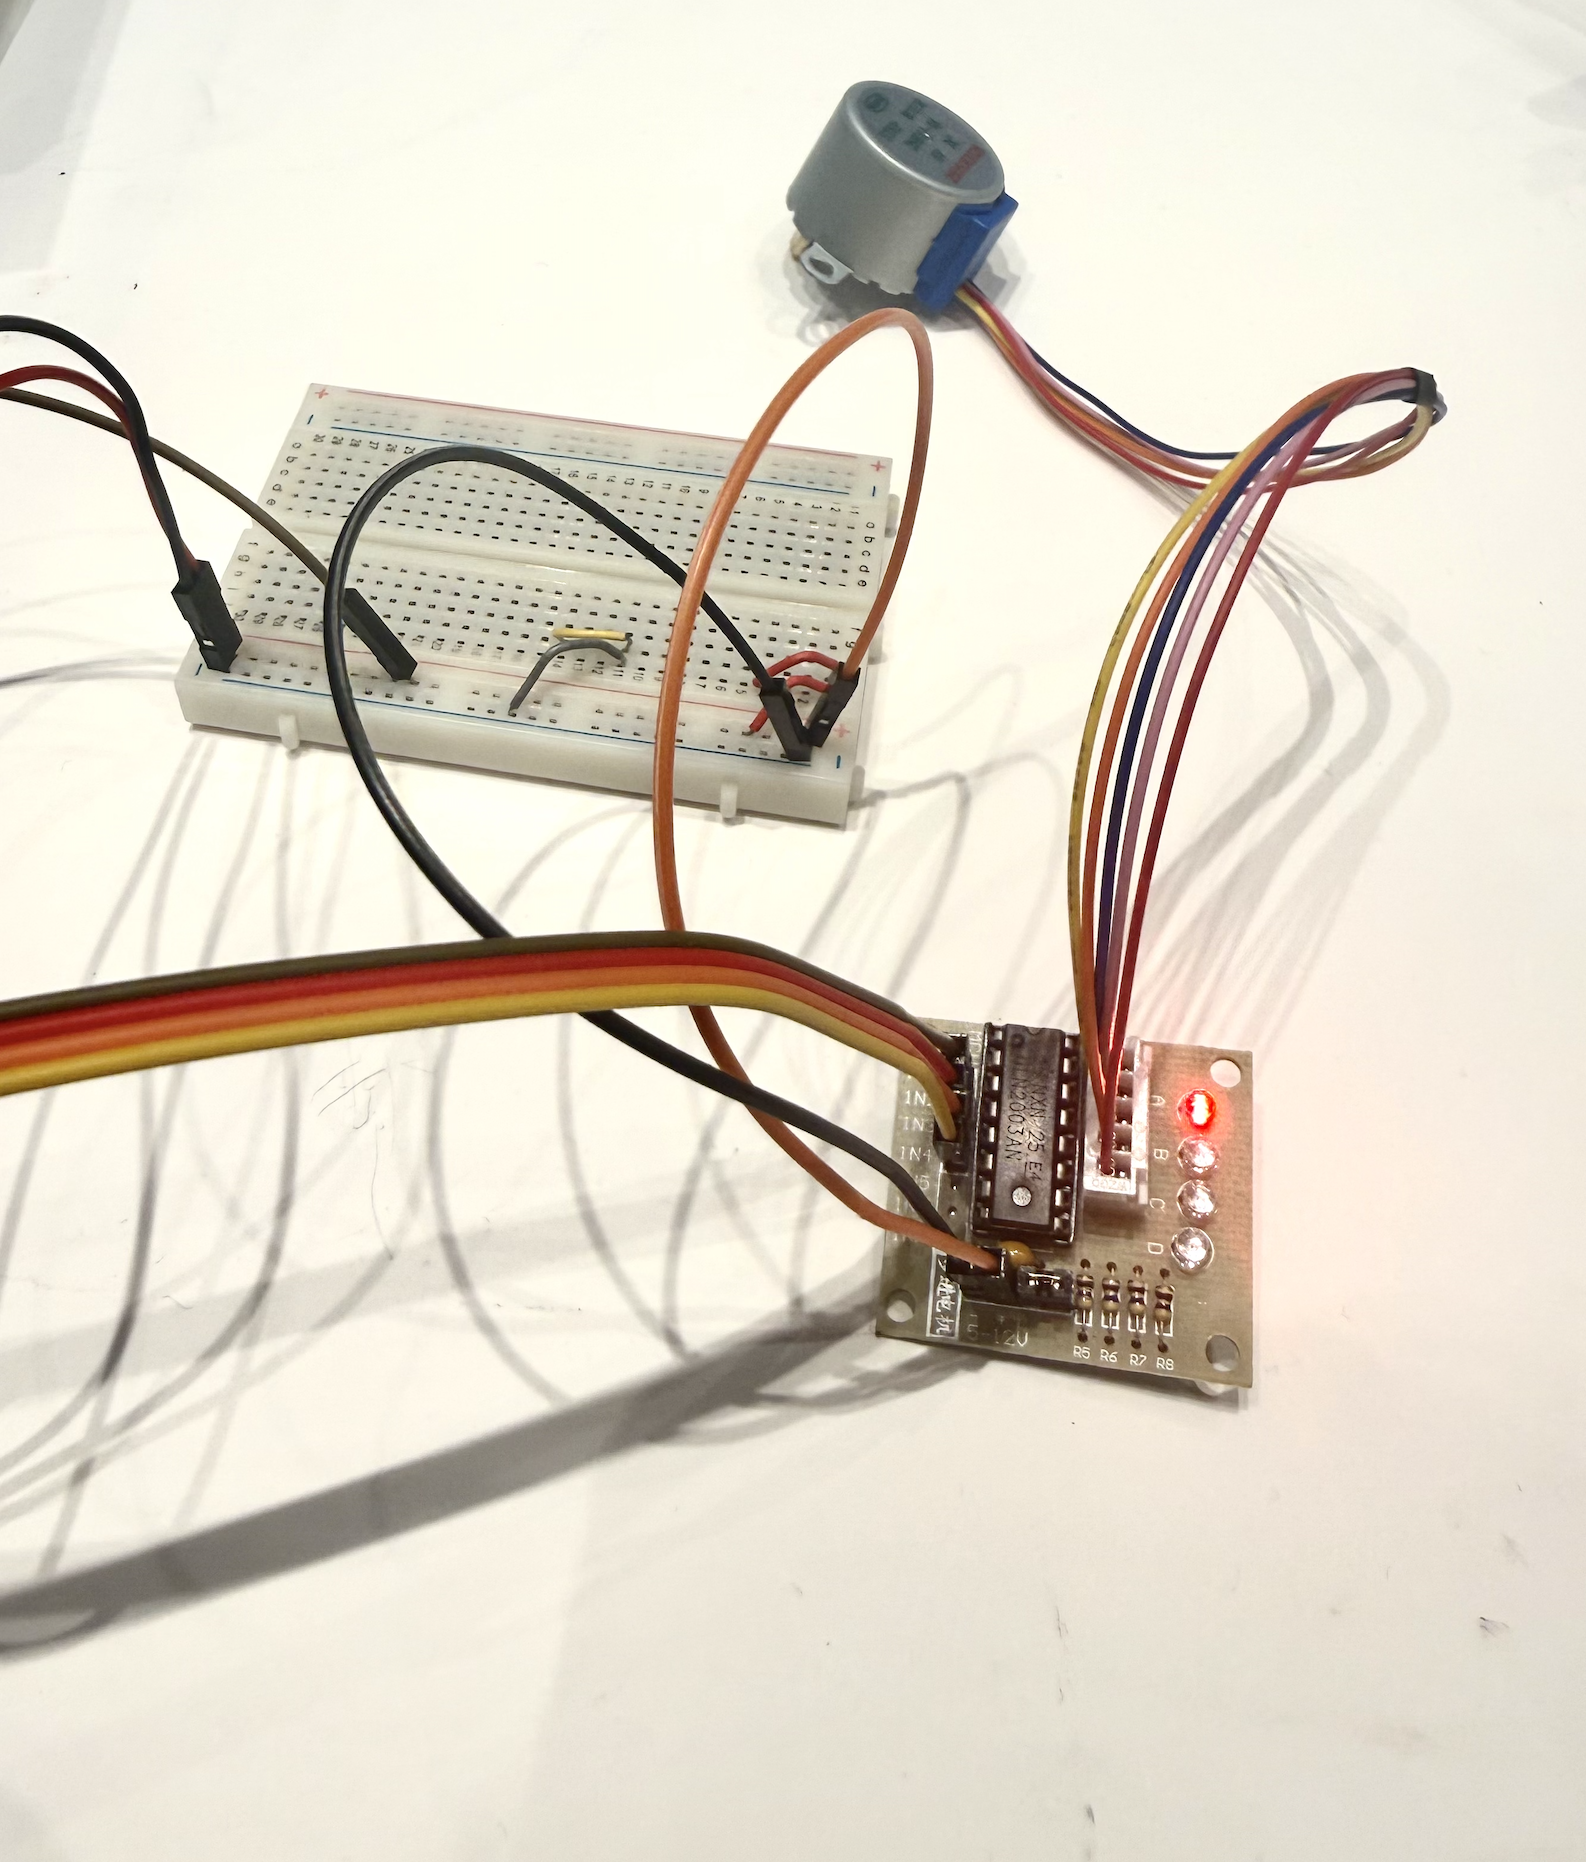
\includegraphics[width=0.4\textwidth]{assets/final/servomotor_driver.png}
        \caption{Perf Board and Servo Motor to Driver Connection}
    \end{figure}

    During the second iteration, several key changes were made to the electrical system. 
    The original 12 V NEMA 17 stepper motors and their corresponding drivers were replaced 
    with 5V 28BYJ-48 stepper motors paired with ULN2003 driver boards. This allowed the 
    removal of the 12 V power supply and enabled the entire system to operate from a single 
    5V source. The wiring diagram was updated accordingly to reflect these component substitutions.

    \section{Third Iteration}
    \subsection{Final Wiring Diagrams}

    \begin{figure}[H]
        \centering
        \includegraphics[width=0.8\textwidth]{assets/third_it/EE_second_wiringdiagrams.png}
        \caption{Final Wiring Diagrams}
    \end{figure}

    \subsection{Final Power Calculations}

    \emph{Per Motor:}

    Approximately 100 mA per coil \* 2 coils \* 5 V \= 1 W
    
    \emph{Raspberry Pi 5:}

    Average consumption of 1.2A \* 5 V \= 6 W
    
    Total System Power:
    \[P_{motor} * 5 + P_{pi} = 1W * 5 = 11W\]

    \subsection{Circuitry}

    \begin{figure}[H]
        \centering
        \includegraphics[width=0.6\textwidth]{assets/final/lidcircuitry.png}
        \caption{Final Circuitry Under Housing Lid}
    \end{figure}

    The only major change from the prototype stage was the transition from breadboard 
    wiring to permanent soldered connections on a perfboard. This improved durability, 
    reduced wiring instability, and prepared the circuitry for integration into the final 
    enclosure.
    

    %===========================FINAL PRODUCT===========================

    \chapter{Final Product}
    \begin{figure}[H]
        \centering
        \includegraphics[width=0.8\textwidth]{assets/final/dispenser.png}
        \caption{Dispenser Systems Fully Assembled}
    \end{figure}
    \begin{figure}[H]
        \centering
        \includegraphics[width=0.8\textwidth]{assets/final/skeleton.png}
        \caption{Skeleton/Internal Structure}
    \end{figure}

    \section{Integration}

    The software portion is hosted by the Raspberry Pi Local hosting and accessed through 
    connecting to a hotspot. The mechanical portion is connected to the Raspberry Pi as shown
    in the wiring diagrams (Figure)

    %===========================DISCUSSION===========================

    \chapter{Discussion}
    
    \section{Limitations and Future Work}

    We discussed in early planning stages the existence of a database
    where users can store pictures they've used in the past, instead of
    taking a new picture every time. We did not complete this for the 
    final project but it would be a consideration for the future. We
    would also consider possible refinements to the algorithm to produce
    even more accurate mixing and image processing. 

    Most of the future work would be to create the features offered on 
    the webpage that we didn't fully develop since they were add ons. 
    We would refine the image processing algorithm so that 
    the user can have an option of uploading a picture with the color 
    reference sheet instead of using the live feed. Another feature that
    we considered was allowing the user to create user profiles to save 
    photos, color recipes, and other data that would allow for a better 
    user experience. 

    %===========================CONCLUSION===========================

    \chapter{Conclusion}

    Our project sucessfully captures a picture, calculates a foundation shade, and dispenses
    a paint mixture close to the shade. Future work would include refining the recipe to ensure
    closer shade matching as well as adding features to the front end to create a better
    user experience. 

    %===========================BILL OF MATERIALS===========================

    \section{Bill of Materials}
    \begin{table}[H]
        \centering
        \begin{tabular}{p{5.5cm} p{5cm} c c}
            \toprule
            Component & Purpose & Qty & Price \\
            \midrule

            2PCS 300mm Tr8x8 Lead Screw + Brass Nut & Linear motion & 3 & \$13.99 \\

            5mm--8mm Lead Screw Coupler (5 pack) & Motor–screw coupling & 1 & \$9.99 \\

            Linear Motion Rod Guide 8mm × 200mm & Linear guidance & 3 & \$8.69 \\

            8mm Flange Pillow Block Bearing & Shaft support & 2 & \$8.99 \\

            Raspberry Pi 5 (4GB RAM) & Main controller & 1 & \$66.00 \\

            5 Pack Plastic 30mL Syringes & Fluid handling prototype & 1 & \$6.99 \\

            Raspberry Pi 5 Power Supply & Power for controller & 1 & \$15.99 \\

            Assorted Metric Fasteners (M2–M5) & Mechanical assembly & 1 & \$20.00 \\

            Limit Switch (10 pack) & Motion limit detection & 1 & \$5.99 \\

            Wiring Kit & Electrical connections & 1 & \$6.98 \\

            5V 3A DC Power Supply & Low-voltage power & 1 & \$7.47 \\

            5 Sets 28BYJ-48 + ULN2003 Driver & Secondary actuation system & 1 & \$14.99 \\

            M2 Spacers & Mechanical spacing & 1 & \$6.69 \\

            Perfboard / Breadboard & Circuit prototyping & 1 & \$8.79 \\

            Mehron Liquid Makeup Colors & Testing material & 1 & \$50.00 \\

            Large 3D Prints (>4 hrs) & Structural components & 1 & \$144.00 \\

            \midrule
            \textbf{Total Estimated Cost} & & & \textbf{\$441.12} \\
            \bottomrule
        \end{tabular}
        \caption{Updated Bill of Materials.}
        \label{tab:hardware_updated}
    \end{table}


    %===========================REFERENCES===========================
    

    \addcontentsline{toc}{chapter}{References}

    \bibliographystyle{unsrt} % Use a numeric style, "unsrt" sorts by order of appearance
    \bibliography{authors} % Name of your .bib file (without the .bib extension)


\end{document}
